\section{Finding Derivatives Algebraically}
\label{sec:algderiv}

\subsection{Formal Limit Definition of the Derivative}

Since a derivative is the slope of a tangent line and a tangent line is the limit of secant lines, we use limits and the formula for the slope of a secant line to find a formula to compute the slope of a tangent line at a point.

The slope of the secant line of $f(x)$ from $x=a$ to $x=b=a+h$ is:
$$\frac{f(b)-f(a)}{b-a}  = \frac{f(a+h)-f(a)}{a+h-a} = \frac{f(a+h)-f(a)}{h}\enspace .$$
As we take $h$ to $0$, we get the slope of the tangent line of $y=f(x)$ at the point $(a, f(a))$.

\begin{definition}[Limit Definition of the Derivative]
\label{def:deriv}
The {\bf derivative}\index{Derivative}\index{Derivative!limit definition} of a function $f(x)$, at the point $(a, f(a))$is:
$$f'(a)=\lim_{h\to 0}\frac{f(a+h)-f(a)}{h} \enspace ,$$
if the limit exists.

The {\bf derivative} of a function $f(x)$, at any point $(x, f(x))$ where $f(x)$ is differentiable is:
$$f'(x)=\lim_{h\to 0}\frac{f(x+h)-f(x)}{h} \enspace .$$
\end{definition}

\begin{example}
Find the slope of the tangent line to $f(x)=\frac{1}{x}$ at $x=3$.

\begin{solution} The slope of the tangent line is the value of the derivative $f'(3)$. $f(3)=\frac{1}{3}$ and $f(3+h)=\frac{1}{3+h}$, so using the limit definition of the derivative, we have:
$$f'(3)=\lim_{h\to 0}\frac{f(3+h)-f(3)}{h}=\lim_{h\to 0}\frac{\frac{1}{3+h}-\frac{1}{3}}{h} \enspace .$$
We can simplify by giving the fractions a common denominator:
\begin{align*}
		\lim_{h\to 0}\frac{\frac{1}{3+h}-\frac{1}{3}}{h}=& \lim_{h\to 0}\frac{\frac{1}{3+h}\cdot\frac{3}{3}-\frac{1}{3}\cdot\frac{3+h}{3+h}}{h} \\
		=& \lim_{h\to 0}\frac{\frac{3}{9+3h}-\frac{3+h}{9+3h}}{h} \\
		=& \lim_{h\to 0}\frac{\frac{3-(3+h)}{9+3h}}{h} \\
		=& \lim_{h\to 0}\frac{\frac{3-3-h}{9+3h}}{h} \\
		=& \lim_{h\to 0}\frac{\frac{-h}{9+3h}}{h} \\
		=& \lim_{h\to 0}\frac{-h}{9+3h}\cdot\frac{1}{h} \\
		=& \lim_{h\to 0}\frac{-1}{9+3h} \enspace .\\
	\end{align*}
Evaluating this using direct substitution, we have:
$$\lim_{h\to 0}\frac{-1}{9+3h}=\frac{-1}{9+3(0)}=-\frac{1}{9} \enspace.$$
Thus, the slope of the tangent line to $f(x)=\frac{1}{x}$ at $x=3$ is $-\frac{1}{9}$.
\end{solution}\end{example}

\begin{example}
Find $\frac{d}{dx}(2x^2-4x-1)$.

\begin{solution} Setting up the derivative using a limit, we have:
$$f'(x)=\lim_{h\to 0}\frac{f(x+h)-f(x)}{h} \enspace .$$
We will start by simplifying $f(x+h)$ by expanding:
\begin{align*}
		f(x+h) &= 2(x+h)^2-4(x+h)-1 \\
		&= 2(x^2+2xh+h^2)-4(x+h)-1 \\
		&= 2x^2+4xh+2h^2-4x-4h-1
	\end{align*}
Now we find the limit as $h$ goes to 0.
\begin{align*}
		f'(x) &= \lim_{h\to 0}\frac{f(x+h)-f(x)}{h} \\
		&= \lim_{h\to 0} \frac{(2x^2+4xh+2h^2-4x-4h-1)-(2x^2-4x-1)}{h} \\
		&= \lim_{h\to 0} \frac{2x^2+4xh+2h^2-4x-4h-1-2x^2+4x+1}{h} \qquad \text{(Substitute in the formulas.)} \\
		&= \lim_{h\to 0} \frac{4xh+2h^2-4h}{h} \qquad \text{(Now simplify.)}\\
		&= \lim_{h\to 0} \frac{h(4x+2h-4)}{h} \qquad \text{(Factor out the \( h \), then cancel.)} \\
		&= \lim_{h\to 0} (4x+2h-4)
	\end{align*}
We can find the limit of this expression by direct substitution:
$$f'(x)=\lim_{h\to 0} (4x+2h-4)=4x-4 \enspace .$$
Notice that the derivative depends on $x$, and that this formula will tell us the slope of the tangent line to $y=f(x)$ at any value $x$. For example, if we wanted to know the tangent slope of $y=f(x)$ at $x=3$, we would simply evaluate: $f'(3)=4\cdot 3-4= 12-4 = 8$.
\end{solution}\end{example}
A formula for the derivative function is very powerful, but as you can see, calculating the derivative using the limit definition is very time consuming. In the next section, we will identify some patterns that will allow us to start building a set of rules for finding derivatives without needing the limit definition.

\subsection{Exercises}
    For each function  $f(x)$  in Problems  \ref{2-5-prob1} - \ref{2-5-prob6}: 
    \begin{enumerate}[label=(\alph*)]
    \item Compute $f'(x)$,
    \item Compute $f'(2)$, and
    \item Find the equation of the line tangent to the graph of $f(x)$ at the point $(2, f(2))$.
    \end{enumerate}

    \begin{enumerate}
    \item $f(x) = 3x - 7$	
    \label{2-5-prob1}
    \item $f(x) = 2 - 7x$	
    \item $f(x) = ax + b$, where  $a$  and  $b$  are constants
    \item $f(x) =  x^2  + 3x$	
    \item $f(x) =  8 - 3x^2$  	
    \item $f(x) = ax^2 + bx + c$,  where $a$, $b$, and $c$ are constants
    \label{2-5-prob6}
    \item Match the graphs of the three functions in Figure \ref{fig:2-5-prob7} with the graphs of their derivatives.
    \begin{figure}[!ht]
  \centering
    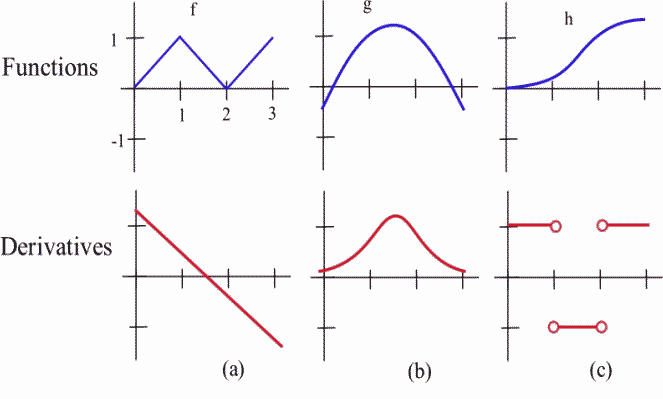
\includegraphics[width=0.4\textwidth]{img/chap2/image032.png}
    \caption{Functions and Derivateives}
    \label{fig:2-5-prob7}
\end{figure}
    \end{enumerate}

